\chapter{Gain-Division Multiple Access}
\label{c:gdma}

In this chapter, we consider the scenario for uplink transmissions over independent fading channels, and the gain-division multiple access (GDMA) with a multiuser detection technique is reviewed for further discussions.

%==================================================

\section{Detection Principle}

A communication system in which $U$ users are sharing the same transmit resource is considered, and the symbol timings of transmissions are assumed to be perfectly aligned. The block diagram of transmitters is shown in Fig.~\ref{fig:gdma_tx}. The message bit sequence ${\bf{d}}_p = [d_u(1), d_u(2), ..., d_u(k)]$ of user-$u$ is encoded into the codeword ${\bf{c}}_u = [c_u(1), c_u(2), ..., c_u(N_c)]$ by an $(N_c,k)$ forward error-correction (FEC) code with code rate $k/N_c$, and the codeword ${\bf{c}}_p$ is then passed to the modulator with order $m$ to get the sequence of modulated symbols ${\bf x}_p = [x_u(1), x_u(2), ..., x_u(N_c/m)]$. The signals of $U$ users are transmitted to the receiver through the independent Rayleigh flat-fading channels, and each of the received symbols in sequence ${\bf r} = [r(1), r(2), ..., r(N_c/m)]$ can be represented as
\begin{align} \label{equ:rx_sup}
 r(n) &= \sum_{u=1}^{U}h_{u}x_{u}(n) + w(n) \nonumber \\ &= s(n) + w(n) ,
\end{align}
where $h_u$ is the channel coefficient between user-$u$ and the receiver, $w(n)$ is the complex additive white Gaussian noise (AWGN) and $s(n)$ is the superimposed symbol consisting of the signals transmitted from $U$ users. There are $2^{mU}$ possible levels in each $s$, where we drop the symbol index $n$ for brevity, and the levels are distinguishable due to the effect of independent fading channels. 

\begin{figure}[t!]
 \centering
 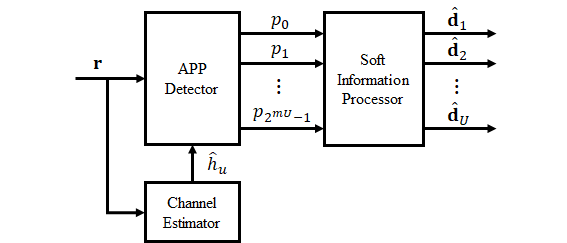
\includegraphics[width=15cm]{fig/gdma_tx.png}
 \caption{Transmitters of $U$ users occupying the same resource.}
 \label{fig:gdma_tx}
\end{figure}

The channel coefficient $h_u$ for a Rician distributed channel can be represented as
\begin{align} \label{equ:rx_sup}
 h_{u} &=\frac{1}{\sqrt{K+1}} \cdot a+\frac{\sqrt{K}}{\sqrt{K+1}}\cdot b \cdot i,
\end{align}

where $a$ and $b$ are normal distribution with variance 1, $a$ is the real part coefficient and $b$ is the imaginary part. $h_{u}$ is the Rayleigh distribution for $K=0$, and Racian distribution for $K\ne0$.


 \begin{figure}[H]
 \centering
 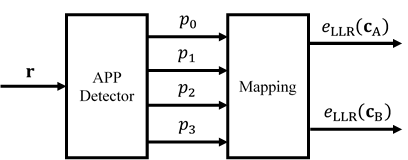
\includegraphics[width=12cm]{fig/gdma_bpsk_u2.png}
 \caption{GDMA detecter for BPSK and $U=2$.}
 \label{fig:gdma_bpsk_u2}
\end{figure}

For the GDMA detector, we divided it into two steps to illustrate.  Firstly, we obtained a $2^{mU}$ dimension probability vector of $a \ posteriori$ probabilities (APPs) for all the superimposed signals. Secondly, Map the $2^{mU}$ dimension probability vector into $U$ Log-likelihood Ratio(LLR). Fig.~\ref{fig:gdma_bpsk_u2} is the block diagram of the GDMA detector in the case of $U = 2$ and BPSK modulation ($m=1$), and the users are denoted as user-A and user-B. The mapping rules for code bits of two users and superimposed levels are tabulated in Table~\ref{table:mapping_m1_p2}, and the possible levels of $s$ are denoted as $S[l]$ with $l \in \{0, 1, 2, 3\}$. In Fig.~\ref{fig:constellation_m1_p2}, a graphical example of the superimposed levels and the corresponding binary mappings $(c_\text{A}, c_\text{B})$ is provided when $h_{\text{A}}$ and $h_{\text{B}}$ are the channel coefficients of user-A and user-B respectively. Note that an accurate estimation of channel coefficients for all users is necessary to recognize the superimposed signal levels properly. In this chapter, we assume that the channel state information (CSI) can be perfectly recovered at the receiver. Thus we can derive all the possible levels of received symbol $s$ for further detection.  

\begin{table}[t!]
\caption{Mapping rules for superimposed signal in the case of $m=1$ and $U=2$.}
\begin{center}
\extrarowheight=2.5pt
\begin{tabular}{|>{\centering\arraybackslash}m{\columnwidth/15}||>{\centering\arraybackslash}m{\columnwidth/10}|>{\centering\arraybackslash}m{\columnwidth/10}||>{\centering\arraybackslash}m{\columnwidth/10}|>{\centering\arraybackslash}m{\columnwidth/10}||>{\centering\arraybackslash}m{\columnwidth/7}|}
\hline 
 $l$ & $c_\text{A}$ & $c_\text{B}$ & $x_\text{A}$ & $x_\text{B}$ &           $S[l]$         \\ \hline
  0  &      0       &      0       &      1       &      1       & $ h_\text{A}+h_\text{B}$ \\ \hline 
  1  &      0       &      1       &      1       &     -1       & $ h_\text{A}-h_\text{B}$ \\ \hline 
  2  &      1       &      0       &     -1       &      1       & $-h_\text{A}+h_\text{B}$ \\ \hline 
  3  &      1       &      1       &     -1       &     -1       & $-h_\text{A}-h_\text{B}$ \\ \hline
\end{tabular}
\label{table:mapping_m1_p2}
\end{center}
\end{table}

\begin{figure}[t!]
 \centering
 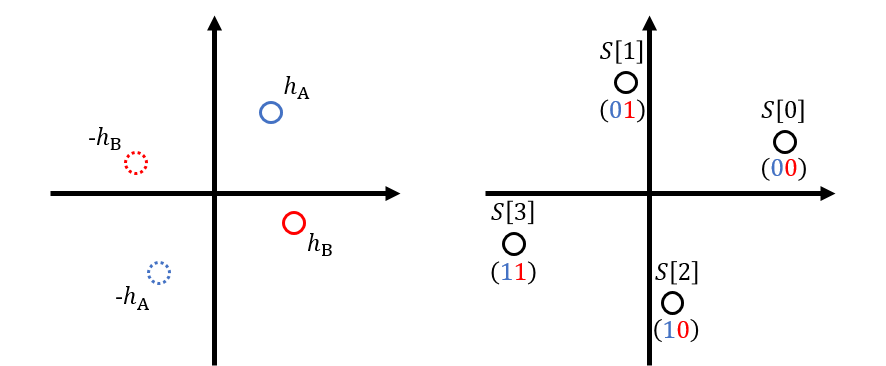
\includegraphics[width=15cm]{fig/constellation_m1_p2.png}
 \caption{An example of superimposed levels in the case of $m=1$ and $U=2$.}
 \label{fig:constellation_m1_p2}
\end{figure}

The $a \ posteriori$ probabilities (APPs) that $s$ is the $l$-th level with $l \in \{0,1,2,3\}$ given the received symbol $r$ can be calculated by
\begin{align}
 p_{l} &= \text{Pr}\left\{s = S[l]\middle|r\right\} \nonumber \\
	   &= \text{Pr}\left\{r\middle|s = S[l]\right\}\cdot\frac{\text{Pr}\left\{s = S[l]\right\}}{\text{Pr}\left\{r\right\}} ,
\label{equ:app} 
\end{align}
and

\begin{align}
 \text{Pr}\left\{r\middle|s = S[l]\right\} = \frac{1}{2\pi{\sigma_w}^{2}}\exp\left(-\frac{\lvert r-S[l]\rvert^{2}}{2{\sigma_w}^{2}}\right) ,
\label{equ:app_2}
\end{align}

where $\text{Pr}\{s = S[l]\}$ is the $a \ priori$ probabilities of $s$ and ${\sigma_w}^2$ is the variance of AWGN. According to the concept of physical layer network coding (PLNC), the APPs of code bits given the received symbol $r$ can be obtained as
\begin{align}
 \text{Pr}\left\{c_\text{A} = 0 \middle| r\right\} &= \text{Pr}\left\{s = S[0]\middle|r\right\} + \text{Pr}\left\{s = S[1]\middle|r\right\} = p_{0} + p_{1}, \nonumber \\
 \text{Pr}\left\{c_\text{A} = 1 \middle| r\right\} &= \text{Pr}\left\{s = S[2]\middle|r\right\} + \text{Pr}\left\{s = S[3]\middle|r\right\} = p_{2} + p_{3},
\end{align}
and
\begin{align}
 \text{Pr}\left\{c_\text{B} = 0 \middle| r\right\} &= \text{Pr}\left\{s = S[0]\middle|r\right\} + \text{Pr}\left\{s = S[2]\middle|r\right\} = p_{0} + p_{2}, \nonumber \\
 \text{Pr}\left\{c_\text{B} = 1 \middle| r\right\} &= \text{Pr}\left\{s = S[1]\middle|r\right\} + \text{Pr}\left\{s = S[3]\middle|r\right\} = p_{1} + p_{3}.
\end{align}

The APPs of code bits can be derived for multiple users with the observation of received superimposed symbols as long as the CSI is available at the receiver. Once the APPs of code bits are obtained, the corresponding log-likelihood ratios (LLRs) of code bits are given by
\begin{align}
 e_{\text{LLR}}(c_\text{A}) = \ln \frac {\text{Pr}\{c_\text{A} = 0|r\}} {\text{Pr}\{c_\text{A} = 1|r\}} = \ln\frac {p_{0}+p_{1}} {p_{2}+p_{3}}, \nonumber \\
 e_{\text{LLR}}(c_\text{B}) = \ln \frac {\text{Pr}\{c_\text{B} = 0|r\}} {\text{Pr}\{c_\text{B} = 1|r\}} = \ln\frac {p_{0}+p_{2}} {p_{1}+p_{3}}.
\label{equ:bit_mapping}
\end{align}


\begin{table}[H]
\caption{Mapping rules for superimposed signal in the case of $m=1$ and $U=3$.}
\begin{center}
\extrarowheight=2pt
\begin{tabular}{|>{\centering\arraybackslash}m{\columnwidth/22}||>{\centering\arraybackslash}m{\columnwidth/14}|>{\centering\arraybackslash}m{\columnwidth/14}|>{\centering\arraybackslash}m{\columnwidth/14}||>{\centering\arraybackslash}m{\columnwidth/14}|>{\centering\arraybackslash}m{\columnwidth/14}|>{\centering\arraybackslash}m{\columnwidth/14}||>{\centering\arraybackslash}m{\columnwidth/5}|}
\hline
 $l$ & $c_1$ & $c_2$ & $c_3$ & $x_1$ & $x_2$ & $x_3$ &     $S[l]$     \\ \hline
  0  &   0   &   0   &   0   &   1   &   1   &   1   & $ h_1+h_2+h_3$ \\ \hline 
  1  &   0   &   0   &   1   &   1   &   1   &  -1   & $ h_1+h_2-h_3$ \\ \hline 
  2  &   0   &   1   &   0   &   1   &  -1   &   1   & $ h_1-h_2+h_3$ \\ \hline 
  3  &   0   &   1   &   1   &   1   &  -1   &  -1   & $ h_1-h_2-h_3$ \\ \hline
  4  &   1   &   0   &   0   &  -1   &   1   &   1   & $-h_1+h_2+h_3$ \\ \hline 
  5  &   1   &   0   &   1   &  -1   &   1   &  -1   & $-h_1+h_2-h_3$ \\ \hline 
  6  &   1   &   1   &   0   &  -1   &  -1   &   1   & $-h_1-h_2+h_3$ \\ \hline 
  7  &   1   &   1   &   1   &  -1   &  -1   &  -1   & $-h_1-h_2-h_3$ \\ \hline
\end{tabular}
\label{table:mapping_m1_p3}
\end{center}
\end{table}

\begin{figure}[t!]
 \centering
 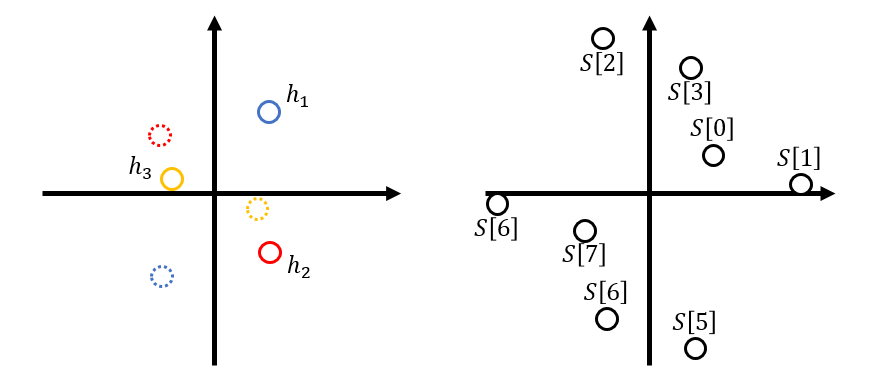
\includegraphics[width=15cm]{fig/constellation_m1_p3.png}
 \caption{An example of superimposed levels in the case of $m=1$ and $U=3$.}
 \label{fig:constellation_m1_p3}
\end{figure}

The multi-level detection technique in GDMA system can be easily extended to the system with $U>2$ and/or $m>1$. For example, in the case of $m=1$ and $U=3$, the mapping rules for code bits of users, denoted as user-1, user-2 and user-3, and superimposed levels are tabulated in Table~\ref{table:mapping_m1_p3}. There are eight possible levels in each superimposed symbol $s$. Let $p_l$ with $l \in \{0,1,...,7\}$ denote the APPs of $s$ given in (\ref{equ:app}), the LLRs of code bits are
\begin{align}
 e_{\text{LLR}}({c}_1) = \ln \frac {\text{Pr}\{c_1 = 0|r\}} {\text{Pr}\{c_1 = 1|r\}} = \ln\frac {p_{0}+p_{1}+p_{2}+p_{3}} {p_{4}+p_{5}+p_{6}+p_{7}}, \nonumber \\
 e_{\text{LLR}}({c}_2) = \ln \frac {\text{Pr}\{c_2 = 0|r\}} {\text{Pr}\{c_2 = 1|r\}} = \ln\frac {p_{0}+p_{1}+p_{4}+p_{5}} {p_{2}+p_{3}+p_{6}+p_{7}}, \nonumber \\
 e_{\text{LLR}}({c}_3) = \ln \frac {\text{Pr}\{c_3 = 0|r\}} {\text{Pr}\{c_3 = 1|r\}} = \ln\frac {p_{0}+p_{2}+p_{4}+p_{6}} {p_{1}+p_{3}+p_{5}+p_{7}}.
\label{equ:p3_llr}
\end{align}


%==================================================

\section{Implementation Methood}

Although the concept of GDMA detection is straightforward, there is no general method to implement the GDMA detector \cite{bh18}\cite{yt19} ,which establishes a mapping table for a specific $U$. With the rise of $U$, the mapping table will grow exponentially, which will significantly improve the complexity of GDMA, and it is challenging to implement. Therefore, we propose a general method that can be implemented more simply and efficiently in this chapter.

\subsection{BPSK-modulated GDMA Implementation}

For general express for BPSK GDMA, we divide the detection into three steps: definition of levels, derivation of APPs ,and derivation of LLRs. Firstly, the superimposed signals $S[l],l\in{1,2,\cdots,L}$ can be express as

\begin{align}
S[1] &= h_{1} + h_{2} + \cdots + h_{U}&={(-1)}^{0} \cdot h_{1}+{(-1)}^{0} \cdot h_{2}+ \cdots + {(-1)}^{0} \cdot h_{U},
 \nonumber \\
S[2] &= h_{1} + h_{2} + \cdots - h_{U}&={(-1)}^{0} \cdot h_{1}+{(-1)}^{0} \cdot h_{2}+ \cdots + {(-1)}^{1} \cdot h_{U}, 
\nonumber \\
\vdots 
\nonumber \\
S[L] &= - h_{1} - h_{2} - \cdots - h_{U}&={(-1)}^{1} \cdot h_{1}+{(-1)}^{1} \cdot h_{2}+ \cdots + {(-1)}^{1} \cdot h_{U}.
\nonumber \\
\end{align}

Convert the decimal $l_{10}$ into binary $l_{2}$, and define $l_{2}$[$u$] is the $u$ -th bit of binary $l_{2}$.  $l_{10} = l_{2} = (l_{2}[1] \quad l_{2}[2] \quad \cdots \quad l_{2}[U])$, $u=1,2,\cdots,U, l_{10} = 0, \cdots, L-1$. We consider that $l_{10}$ is the serial number to record superimposed levels and consider that $l_2[u]$ is the code bit for user-$u$. Moreover, $l_2[u]$ is also a mapping index for $u$-user's channel gain $h_u$. We can derive mapping index from $S[l]$ directly by converting from decimal to binary. In the following expression, $l_{10}$ and $l_2$ are used alternately.

\begin{align}
S[l_{10}] &={(-1)}^{l_{2}[1]} \cdot h_{1}+{(-1)}^{l_{2}[U]} \cdot h_{2}+ \cdots + {(-1)}^{l_{2}[U]} \cdot h_{U} 
\nonumber \\
&= \sum_{u=1}^{U} (-1)^{l_2[u]} \cdot h_u, l_{10} = 0, 1, \cdots, L-1 
\label{equ:implementation_1}
\end{align}
where $h_{u}$ is the complex channel coefficient of user-$u$. Secondly, APPs of $l$-th level with $l\in{0,1,2,\cdots,L}$ given the received symbol $r$ can be calculated as equation.\ref{equ:app}. Thirdly, once the APPs are obtained, the mapping formula can be expressed as 

\begin{align}
e_{\text{LLR}}[c_u] &= ln \frac{\text{Pr}\{c_u=0|r\}}{\text{Pr}\{c_u=1|r\}}
\nonumber \\
&= ln \frac{\sum_{l_{10}=0, l_{2}[u]\in{0}}^{L}\text{Pr}\{s=S[l]|r\}}{\sum_{l_{10}=0, l_{2}[u]\in{1}}^{L}\text{Pr}\{s=S[l]|r\}}
\label{equ:implementation_2}
\end{align}

\begin{figure}[b!]
 \centering
 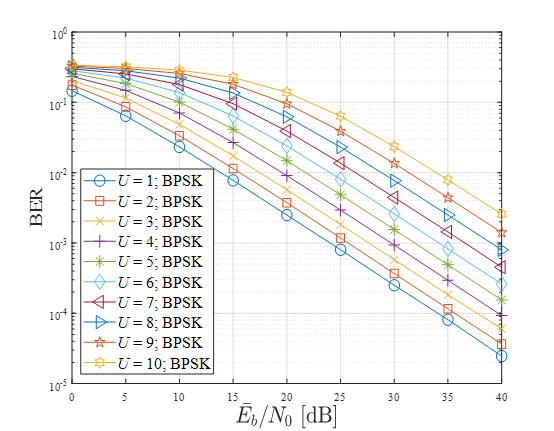
\includegraphics[width=15cm]{fig/gdma_bpsk_implement_u2.png}
 \caption{BER performances of uncoded GDMA BPSK system over block Rayleigh fading channels.}
 \label{fig:bpsk_implementation}
\end{figure}

The two equations above and below the fraction are the probability that user-$u$ code bits are equal to zero or one, and there are $\frac{L}{2}$ APPs added respectively. The APPs of the upper fraction must meet $h_u$ superimposition, and the APPs of the lower fraction must meet $-h_u$ superimposition. According to \ref{equ:implementation_1}, we can use mapping index $l_2[u]$ equal to zero or one to judge whether meet the $u$-user restriction.



\subsection{QPSK-modulated GDMA Implementation}

 In addition to BPSK, we also discuss the general detection of QPSK with modulation order ($m=2$). According to QPSK modulation, the superimposed signals $S[l],l\in{1,2,\cdots,L}$ can be expressed as
\begin{align}
S[0] &= e^{\frac{\pi}{4}j}h_{1} + e^{\frac{\pi}{4}j}h_{2} + \cdots + e^{\frac{\pi}{4}j}h_{U},
\nonumber \\
S[1] &= e^{\frac{\pi}{4}j}h_{1} + e^{\frac{\pi}{4}j}h_{2} + \cdots + e^{(\frac{\pi}{4}+\frac{\pi}{2})j}h_{U},
\nonumber \\
S[2] &= e^{\frac{\pi}{4}j}h_{1} + e^{\frac{\pi}{4}j}h_{2} + \cdots + e^{(\frac{\pi}{4}+\pi)j}h_{U},
\nonumber \\
S[3] &= e^{\frac{\pi}{4}j}h_{1} + e^{\frac{\pi}{4}j}h_{2} + \cdots + e^{(\frac{\pi}{4}+\frac{3\pi}{2})j}h_{U},
\nonumber \\
\vdots 
\nonumber \\ \nonumber \\
S[L-1] &= e^{(\frac{\pi}{4}+\frac{3\pi}{2})j}h_{1} + e^{(\frac{\pi}{4}+\frac{3\pi}{2})j}h_{2} + \cdots + e^{(\frac{\pi}{4}+\frac{3\pi}{2})j}h_{U}.
\label{equ:implementation_4}
\end{align}

Different from BPSK detection, we convert the decimal $l_{10}$ into quaternary $l_{4}$ since the modulation order $(m=2)$, and define that $l_{4}[u]$ is the $u$-th bit of quaternary $l_{4}$. $l_{10}=l_{4}=(l_4[1]  \quad l_4[2] \quad  \cdots \quad  l_4[U]),u=1,2,\cdots U$.  We consider that $l_4[u]$ is the code symbol for user-$u$, which might be 00, 01, 10, 11. Moreover, $l_4[u]$ is also a mapping index for $u$-user's channel gain $h_u$. After simplifying \ref{equ:implementation_4}, we can obtain superimposed levels as

\begin{align}
S[l] &= e^{(\frac{\pi}{4} + \frac{\pi}{2} \cdot l_{4}[1])j} \cdot h_{1} + e^{(\frac{\pi}{4} + \frac{\pi}{2} \cdot l_{4}[1])j} \cdot h_{2} + \cdots + e^{(\frac{\pi}{4} + \frac{\pi}{2} \cdot l_{4}[1])j} \cdot h_{U} 
\nonumber \\
&= \sum_{u=1}^{U}e^{(\frac{\pi}{4} + \frac{\pi}{2} \cdot l_{4}[u])j} \cdot h_{u}, l_{10}= 0, 1, \cdots, L-1; u=1, 2, \cdots, U
\label{equ:qpsk_level_define}
\end{align}

In the above definition \ref{equ:qpsk_level_define}, we can define levels architecturally, and then need to derive the APP of each level. The 
APPs can be calculated as \ref{equ:app}. Finally,  $e_{\text{LLR}}$ can be easily obtained with the structure of $S[l]$.

\begin{equation}
e_{\text{LLR}}[c_u] = ln \frac{\text{Pr}\{c_u=0|r\}}{\text{Pr}\{c_u=1|r\}} 
\nonumber \\ = 
\left\{
             \begin{array}{lr}
             ln \frac{\sum_{l_{10}=0, l_{2}[u]\in\{0,1\}}^{L}\text{Pr}\{s=S[l]|r\}}{\sum_{l_{10}=0, l_{2}[u]\in\{2,3\}}^{L}\text{Pr}\{s=S[l]|r\}}, i = 1; u=1,\cdots, U &  \\
             ln \frac{\sum_{l_{10}=0, l_{2}[u]\in\{0,2\}}^{L}\text{Pr}\{s=S[l]|r\}}{\sum_{l_{10}=0, l_{2}[u]\in\{1,3\}}^{L}\text{Pr}\{s=S[l]|r\}},
i = 2; u=1,\cdots, U & \\ 
             \end{array}
\right.
\label{equ:implementation_3}
\end{equation}

	The Fig.\ref{fig:qpsk_gray_mapping} is the QPSK constellation according to gray mapping. We need to consider the code bit code bits corresponding to the first or the second bit on constellation. For first bit $i=1$, both level-$S[0]$ and level-$S[1]$ are mapping to code bit equal to $0$, while level-$S[2]$ and level-$S[3]$ are mapping to code bits equal to $1$, where $i=1,\cdots, m$ is the $i$-bit for constellation. We also can use mapping index $l_{4}[u]$ to extract the phase information from $S[l]$. Map LLR according to $i$-constellation location and $u$-user. 
	
	Fig.\ref{fig:qpsk_implementation} is the BER performance of uncoded GDMA QPSK over a block rayleigh fading channel.

\begin{figure}
 \centering
 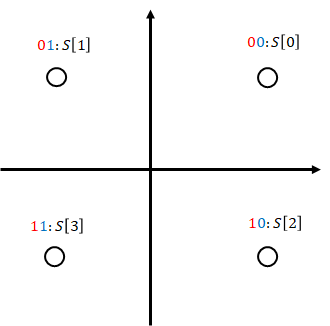
\includegraphics[width=7cm]{fig/qpsk_gray_mapping.png}
 \caption{QPSK modulation gray mapping.}
 \label{fig:qpsk_gray_mapping}
\end{figure}

\begin{figure}[H]
 \centering
 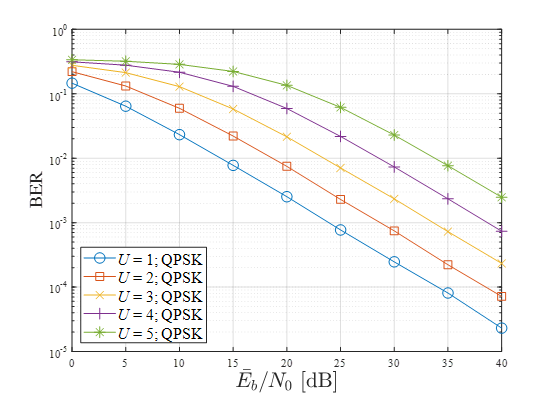
\includegraphics[width=15cm]{fig/gdma_qpsk_implement.png}
 \caption{BER performances of uncoded GDMA QPSK system over block Rayleigh fading channels.}
 \label{fig:qpsk_implementation}
\end{figure}

\subsection{PAM-modulated GDMA Implementation}

Consider a general PAM case: $2^m$-PAM; $U$ is integer; $m$ is integer; $E_v$  is the average power; $M=2^m-1$ is the mid number.

The superimposed signals $S[l],l\in{1,2,\cdots,L}$ can be express as
\begin{align}
S[0] &= (2 \cdot 0-M)\cdot\sqrt{E_s}\cdot h_1 + (2\cdot0 - M)\cdot\sqrt{E_s}\cdot h_2 +, \cdots + (2 \cdot 0-M)\cdot\sqrt{E_s}\cdot h_U,
\nonumber \\
S[1] &= (2 \cdot 0-M)\cdot\sqrt{E_s}\cdot h_1 + (2\cdot0 - M)\cdot\sqrt{E_s}\cdot h_2 +, \cdots + (2 \cdot 1-M)\cdot\sqrt{E_s}\cdot h_U,
\nonumber \\
S[2] &= (2 \cdot 0-M)\cdot\sqrt{E_s}\cdot h_1 + (2\cdot0 - M)\cdot\sqrt{E_s}\cdot h_2 +, \cdots + (2 \cdot 2-M)\cdot\sqrt{E_s}\cdot h_U,
\nonumber \\
S[3] &= (2 \cdot 0-M)\cdot\sqrt{E_s}\cdot h_1 + (2\cdot0 - M)\cdot\sqrt{E_s}\cdot h_2 +, \cdots + (2 \cdot 3-M)\cdot\sqrt{E_s}\cdot h_U,
\nonumber \\
\vdots 
\nonumber \\ 
S[L-1] &= (2 \cdot M-M)\cdot\sqrt{E_s}\cdot h_1 + (2\cdot M - M)\cdot\sqrt{E_s}\cdot h_2 +, \cdots + (2 \cdot M-M)\cdot\sqrt{E_s}\cdot h_U.
\label{equ:implementation_5}
\end{align}

We can convert the decimal $l_{10}$ into quaternary $l_{M}$, and define that $l_{M}[u]$ is the $u$-th bit of $l_{M}$. $l_{10}=l_{M}=(l_M[1]  \quad l_M[2] \quad  \cdots \quad  l_M[U]),u=1,2,…U$. After simplifying \ref{equ:implementation_5}, we can obtain superimposed levels as

\begin{align}
S[l] &= (2 \cdot l_{2^{m}}[1]-M)\cdot\sqrt{E_v}\cdot h_1 + (2 \cdot l_{2^{m}}[2]-M)\cdot\sqrt{E_v}\cdot h_2 +, \cdots + (2 \cdot l_{2^{m}}[U]-M)\cdot\sqrt{E_v}\cdot h_U
\nonumber \\
&= \sum_{u=1}^{U}(2\cdot l_{2^{m}}[u]-M)\cdot\sqrt{E_{v}}\cdot h_u, u=1,2, \cdots, U
\end{align}

In the above definition, we can define levels architecturally and then need to derive the APP of each level. The APPs can be calculated as \ref{equ:app}. Finally,  $e_{\text{LLR}}$ can be easily obtained with the structure of $S[l]$. According to m, there will be different gray mapping for PAM. Firstly, we discuss the 4-PAM and the gray mapping in Fig.\ref{fig:4_pam_gray_mapping}. 

\begin{figure}
 \centering
 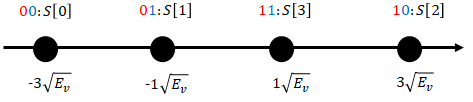
\includegraphics[width=10cm]{fig/4_pam_gray_mapping.png}
 \caption{4-PAM modulation gray mapping.}
 \label{fig:4_pam_gray_mapping}
\end{figure}

\begin{equation}
e_{\text{LLR}}[c_u] = ln \frac{\text{Pr}\{c_u=0|r\}}{\text{Pr}\{c_u=1|r\}} 
\nonumber \\ = 
\left\{
             \begin{array}{lr}
             ln \frac{\sum_{l_{10}=0, l_{4}[u]\in\{0,1\}}^{L}\text{Pr}\{s=S[l]|r\}}{\sum_{l_{10}=0, l_{4}[u]\in\{2,3\}}^{L}\text{Pr}\{s=S[l]|r\}}, i = 1; u=1,\cdots, U &  \\
             ln \frac{\sum_{l_{10}=0, l_{4}[u]\in\{0,3\}}^{L}\text{Pr}\{s=S[l]|r\}}{\sum_{l_{10}=0, l_{4}[u]\in\{1,2\}}^{L}\text{Pr}\{s=S[l]|r\}},
i = 2; u=1,\cdots, U & \\ 
             \end{array}
\right.
\end{equation}

Secondly, we discuss the 8-PAM and the gray mapping \ref{fig:8_pam_gray_mapping}. 

\begin{figure}
\centering
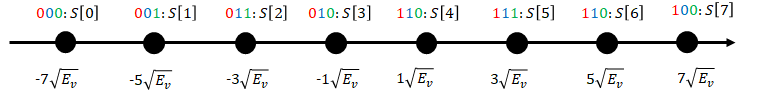
\includegraphics[width=17cm]{fig/8_pam_gray_mapping.png}
\caption{8-PAM modulation gray mapping.}
\label{fig:8_pam_gray_mapping}
\end{figure}

\begin{equation}
e_{\text{LLR}}[c_u] = ln \frac{\text{Pr}\{c_u=0|r\}}{\text{Pr}\{c_u=1|r\}} 
\nonumber \\ = 
\left\{
             \begin{array}{lr}
             ln \frac{\sum_{l_{10}=0, l_{8}[u]\in\{0,1,2,3\}}^{L}\text{Pr}\{s=S[l]|r\}}{\sum_{l_{10}=0, l_{8}[u]\in\{4,5,6,7\}}^{L}\text{Pr}\{s=S[l]|r\}}, i = 1; u=1,\cdots, U &  \\
             ln \frac{\sum_{l_{10}=0, l_{8}[u]\in\{0,1,6,7\}}^{L}\text{Pr}\{s=S[l]|r\}}{\sum_{l_{10}=0, l_{8}[u]\in\{2,3,4,5\}}^{L}\text{Pr}\{s=S[l]|r\}},
i = 2; u=1,\cdots, U & \\
			ln \frac{\sum_{l_{10}=0, l_{8}[u]\in\{0,3,4,7\}}^{L}\text{Pr}\{s=S[l]|r\}}{\sum_{l_{10}=0, l_{8}[u]\in\{1,2,5,6\}}^{L}\text{Pr}\{s=S[l]|r\}},
i = 2; u=1,\cdots, U & \\ 
             \end{array}
\right.
\end{equation}

\begin{figure}[t!]
 \centering
 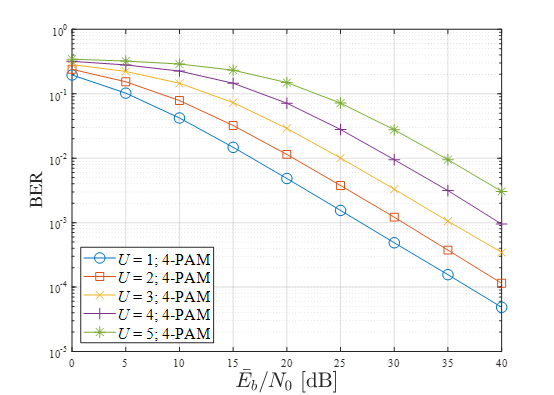
\includegraphics[width=15cm]{fig/gdma_4_PAM_implement.png}
 \caption{BER performances of uncoded GDMA 4-PAM system over block Rayleigh fading channels.}
 \label{fig:4_pam_implementation}
\end{figure}

\begin{figure}[t!]
 \centering
 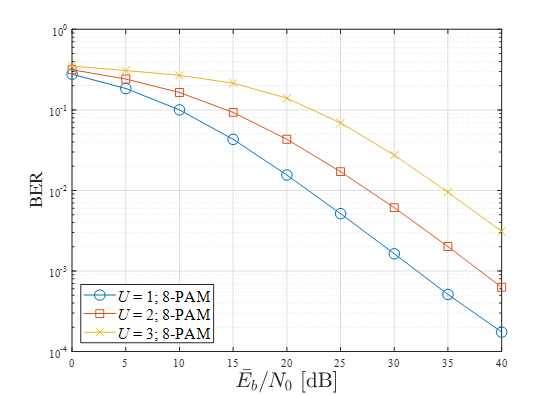
\includegraphics[width=15cm]{fig/gdma_8_PAM_implement.png}
 \caption{BER performances of uncoded GDMA 8-PAM system over block Rayleigh fading channels.}
 \label{fig:8_pam_implementation}
\end{figure}

Fig.\ref{fig:4_pam_implementation} and fig.\ref{fig:8_pam_implementation} are the BER performance respectively for uncoded GDMA 4-pam and 8-pam.


\begin{figure}[H]
 \centering
 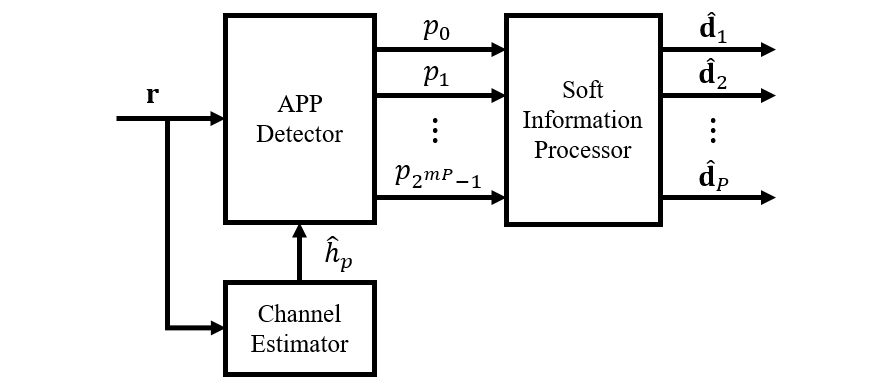
\includegraphics[width=15cm]{fig/gdma_rx.png}
 \caption{Multi-level receiver in GDMA system for recovering the messages of U users.}
 \label{fig:gdma_rx}
\end{figure}


The LLRs can be directly used for data detection or be further fed to the following soft information processor (SIP) when FEC coding is considered. The block diagram of the multiuser detector in GDMA system is shown in Fig.~\ref{fig:gdma_rx}. The SIP can be implemented by using several decoders (DECs) and one for each user independently as shown in Fig.~\ref{fig:gdma_scd}. A joint channel decoder can be an alternative to implement the SIP and extract the messages of all users simultaneously. The implementation of SIP will be discussed in Sec.~\ref{s:mldt_fec}. 
If the messages are transmitted without FEC coding, the decision rule with the APPs derived from multi-level detection is equivalent to finding the nearest neighbor of received symbol among all the levels. The corresponding decision region depends on the channel coefficients.

\begin{figure}[H]
 \centering
 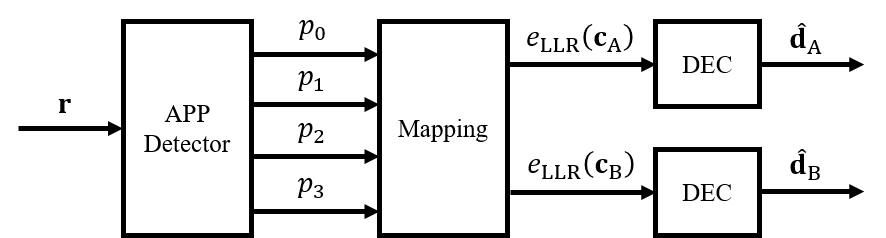
\includegraphics[width=15cm]{fig/gdma_scd.png}
 \caption{Separated channel decoding in the case of $m=1$ and $U=2$.}
 \label{fig:gdma_scd}
\end{figure}

%==================================================
\section{Joint channel decoding for the GDMA system}
\label{s:mldt_fec}

In this section, the implementation flow of the soft information processor (SIP) in the multiuser detector is discussed. We firstly review the joint channel decoding for the LDPC coded GDMA system and secondly discuss a novel joint channel decoding for the polar coded system.

%--------------------------------------------------

\subsection{Introduction of Joint Channel Decoding}

A straightforward method to construct the SIP in GDMA system is called separated channel decoding (SCD) as shown in fig.~\ref{fig:gdma_scd}. To recover the messages of $U$ users in GDMA-SCD system, the APPs of code bits are first attained and then be fed to the following decoders independently for each user. Note that there is no exchange of informations between collided users in GDMA-SCD scheme.

Another method of FEC-GDMA system is called Joint Channel Decoding (JCD) as shown in \ref{fig:gdma_jcd}, an alternative to implement the SIP in the case of $U=2$ and BPSK transmission. In the GDMA-JCD system, The APPs of codeword will pass the message to the JCD decoder before mapping LLRs. In the JCD, $L$ APP vectors will pass to JCD decoder, therefore, the APPs will be more reliable. However, the amount of messages passing is $L$ times of SCD, the operation complexity will be an exponentially increase.


\begin{figure}[t!]
 \centering
 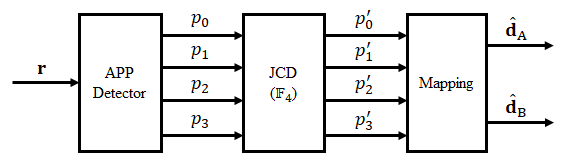
\includegraphics[width=15cm]{fig/gdma_jcd.png}
 \caption{Joint channel decoding in the case of $m=1$ and $U=2$.}
 \label{fig:gdma_jcd}
\end{figure}

\subsection{LDPC Coded GDMA system}

A generalized joint channel decoding and physical-layer network coding (G-JCNC) in \cite{gjcnc10}. The G-JCNC was proposed to combine the soft decoding of LDPC codes and the physical-layer network coding (PLNC), and here we take advantage of joint channel decoding (JCD) to extract the messages of $U$ users simultaneously. The APPs of each symbol $s(n)$, $p_l$ with $l \in \{0, 1, ..., 2^{mU}-1\}$, are sent to a non-binary decoder using generalized SPA (G-SPA), and the decoding is performed with respect to $\mathbb{F}_{2^{mU}}$. The procedure of G-SPA in the case of $U=2$ and BPSK transmission is described as follows.


\paragraph{Messages and Initialization}

An LDPC code can be represented as a bipartite graph, called Tanner graph, defined by the parity-check matrix with two kinds of nodes: check nodes and variable nodes. The G-SPA iteratively determines the APPs of the symbol $s(n)$ with $n \in \{1, 2, ..., N_c\}$ over the Tanner graph \cite{spa01}. The four possible levels in each $s(n)$ are shown in Table~\ref{table:mapping_m1_p2}. The message passed through the edges in the corresponding Tanner graph are represented by probability vector ${\bf p} = [ \ p_0 \ p_1 \ p_2 \ p_3 \ ]$ where $p_i$ is the probability that the value of variable $s(n)$ is $S[l]$ with $l \in \{0, 1, 2, 3\}$, and $ p_0+p_1+p_2+p_3=1$ holds. The initial message of variable node $s(n)$ given the received symbol $r(n)$ is $p_{l} = \text{Pr}\left\{s(n) = S[l]\middle|r\right\}$ with $l \in \{0, 1, 2, 3\}$ given in (\ref{equ:app}). 

The message updating rules at variable nodes and check nodes within the G-SPA are the same as that discussed in \cite{spa01}, and the update functions are defined as $\text{VAR}$ and $\text{CHK}$ for variable nodes and check nodes respectively. The discussion is restricted to nodes of degree three and the messages from the nodes with degree greater than three can be calculated by
\begin{align}
 \text{VAR}({\bf p}, {\bf q}, \cdots) & = {\textrm{VAR}}({\bf p}, {\textrm{VAR}}({\bf q}, {\textrm{VAR}}(\cdot, \cdot))) , \nonumber \\
 \text{CHK}({\bf p}, {\bf q}, \cdots) & = {\textrm{CHK}}({\bf p}, {\textrm{CHK}}({\bf q}, {\textrm{CHK}}(\cdot, \cdot))) ,
\end{align}
where ${\bf p}$ and ${\bf q}$ denote the corresponding input messages derived from variable nodes or check nodes. The functions of $\text{VAR}$ and $\text{CHK}$ at the nodes of degree three are illustrated in Fig.~\ref{fig:gspa_msg}, and the circles and squares represent the variable nodes and check nodes respectively. 

\begin{figure}[b!]
 \centering
 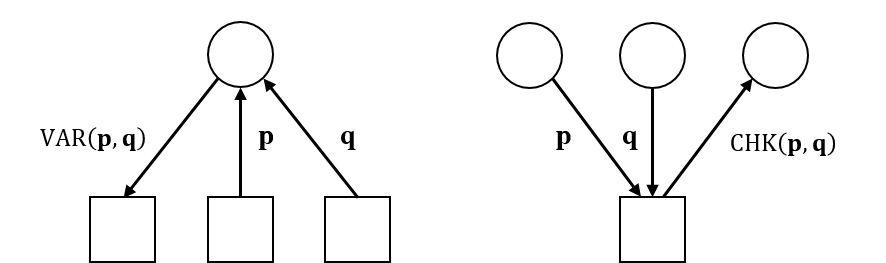
\includegraphics[width=15cm]{fig/gspa_msg.png}
 \caption{The message passing algorithm along the edges in factor graph.}
 \label{fig:gspa_msg}
\end{figure}

\paragraph{Output Message of Variable Nodes}

When the two input messages ${\bf p} = [ \ p_0 \ p_1 \ p_2 \ p_3 \ ]$ and ${\bf q} = [ \ q_0 \ q_1 \ q_2 \ q_3 \ ]$ arrive at the variable node $s(n)$, the probability that $s(n)=S[l]$ with $l \in \{0 ,1, 2, 3\}$ is given by
\begin{align}
 \text{Pr}\{s(n)=S[l]|{\bf p}, {\bf q}\} & = \frac{\text{Pr}\{{\bf p}, {\bf q}|s(n)=S[l]\}\text{Pr}\{s(n)=S[l]\}}{\text{Pr}\{{\bf p}, {\bf q}\}} \nonumber \\
 & = \frac{\text{Pr}\{s(n)=S[l]|{\bf p}\}\text{Pr}\{s(n)=S[l]|{\bf q}\}\text{Pr}\{{\bf p}\}\text{Pr}\{{\bf q}\}}{\text{Pr}\{{\bf p}, {\bf q}\}} \nonumber \\
 & = \beta p_l q_l ,
\end{align}
where
\begin{align}
 \beta = \frac{\text{Pr}\{{\bf p}\}\text{Pr}\{{\bf q}\}}{\text{Pr}\{{\bf p}, {\bf q}\}} = \frac{1}{p_0 q_0 + p_1 q_1 + p_2 q_2 + p_3 q_3} ,
\end{align}
is a normalization factor. Therefore, the output message of variable node $s(n)$ is
\begin{align}
 \text{VAR}({\bf p}, {\bf q}) = \beta [ \ p_0 q_0 \ p_1 q_1 \ p_2 q_2 \ p_3 q_3 \ ] .
\end{align}

\paragraph{Output Message of Check Nodes}

A specific parity-check equation is satisfied if the $\mathbb{F}_4$ sum of the connected quaternary symbols in the corresponding Tanner graph is equal to zero, i.e., $s(n) \oplus s(n_1) \oplus s(n_2) = 0$. Assuming that the two input messages derived from the variable nodes $s(n_1)$ and $s(n_2)$ are ${\bf p} = [ \ p_0 \ p_1 \ p_2 \ p_3 \ ]$ and ${\bf q} = [ \ q_0 \ q_1 \ q_2 \ q_3 \ ]$, respectively. The probability that the parity-check equation is satisfied under the the assumption that $s(n)=S[0]$ is
\begin{align}
 \text{Pr}\{s(n)=S[0]|{\bf p}, {\bf q}\} = & \quad \text{Pr}\{s(n_1)=S[0], s(n_2)=S[0]|{\bf p}, {\bf q}\} \nonumber \\
 & + \text{Pr}\{s(n_1)=S[1], s(n_2)=S[1]|{\bf p}, {\bf q}\} \nonumber \\
 & + \text{Pr}\{s(n_1)=S[2], s(n_2)=S[2]|{\bf p}, {\bf q}\} \nonumber \\
 & + \text{Pr}\{s(n_1)=S[3], s(n_2)=S[3]|{\bf p}, {\bf q}\} \nonumber \\
 = & \quad p_0 q_0 + p_1 q_1 + p_2 q_2 + p_3 q_3.
\end{align}
Similarly we can have
\begin{align}
 \text{Pr}\{s(n)=S[1]|{\bf p}, {\bf q}\} & = p_0 q_1 + p_1 q_0 + p_2 q_3 + p_3 q_2, \nonumber \\
 \text{Pr}\{s(n)=S[2]|{\bf p}, {\bf q}\} & = p_0 q_2 + p_2 q_0 + p_1 q_3 + p_3 q_1, \nonumber \\
 \text{Pr}\{s(n)=S[3]|{\bf p}, {\bf q}\} & = p_0 q_3 + p_3 q_0 + p_1 q_2 + p_2 q_1.
\end{align}
Finally, the message out of one check node equals
\begin{equation}
 \text{CHK}({\bf p},{\bf q})= \left[
 \begin{split}
  &p_0 q_0 + p_1 q_1 + p_2 q_2 + p_3 q_3 \\
  &p_0 q_1 + p_1 q_0 + p_2 q_3 + p_3 q_2 \\
  &p_0 q_2 + p_2 q_0 + p_1 q_3 + p_3 q_1 \\
  &p_0 q_3 + p_3 q_0 + p_1 q_2 + p_2 q_1
 \end{split}
 \right]^T.
\end{equation}

\paragraph{Finalization and Symbol-to-Bit Mapping}

The decoding algorithm is stopped if all parity-check equations are fulfilled or the maximum number of iterations is reached. Otherwise, the process proceed with further iteration until one of the conditions is satisfied. At the end of the decoding algorithm, the G-SPA generates the APP vector ${\bf p} = [ \ p_0 \ p_1 \ p_2 \ p_3 \ ]$  with $p_i = \text{Pr}\left\{s(n) = S[l]\middle|r\right\}$ for each symbol $s(n)$ with $n \in \{1, 2, ..., N_c\}$ and the symbol-to-bit mapping is done by (\ref{equ:bit_mapping}). The combination of multi-level detection and G-SPA is referred to as GDMA-JCD scheme in this thesis. The G-SPA with higher-order modulation scheme was investigated in \cite{gjcncqpsk10}. 

\paragraph{Simulation Results} 

The BLER performances of GDMA-JCD and GDMA-SCD systems using a (1008, 504) rate-1/2 binary (3,6)-regular LDPC code with BPSK transmissions over quasi-static Rayleigh flat-fading channels are provided in Fig.~\ref{fig:bler_ldpc}. The maximum number of decoding iterations is set to 50 for both SPA and G-SPA. In the transmissions over block flat-fading channels, the GDMA-JCD scheme outperforms the GDMA-SCD scheme in low-SNR region and the performances of two schemes converge to each other in high-SNR region. We further consider an OFDM-GDMA system that has $16$ sub-carrier and $63$ bits for each sub-carrier symbol. The BLER performance of GDMA-OFDM-JCD and GDMA-OFDM-SCD using same parameters as above and are provided in Fig.~ \ref{fig:bler_ofdm_ldpc}. We found that JCD can effectively use different user information, even when increasing the number of users, performance has almost no loss.


\begin{figure}[t!]
 \centering
 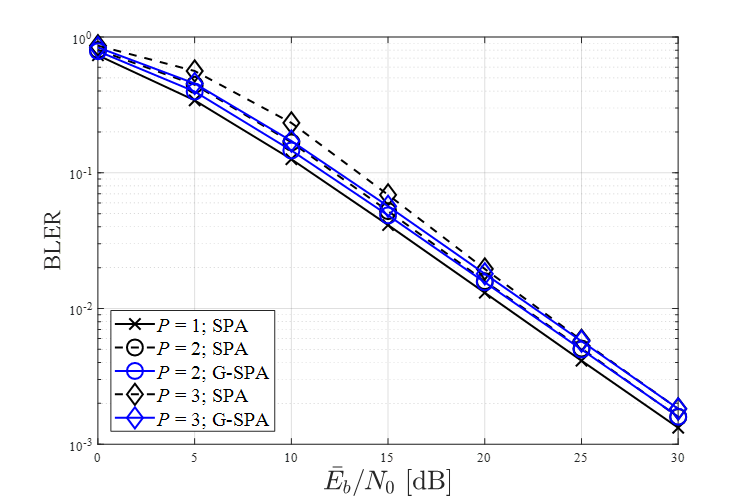
\includegraphics[width=14cm]{fig/bler_ldpc.png}
 \caption{BLER performances of (1008, 504) LDPC-coded GDMA systems over quasi-static Rayleigh flat-fading channels.}
 \label{fig:bler_ldpc}
\end{figure}

\begin{figure}[b!]
 \centering
 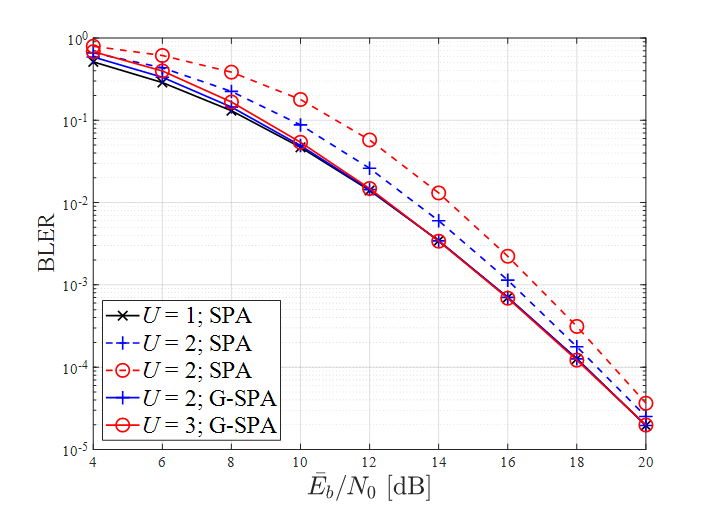
\includegraphics[width=14cm]{fig/bler_gdma_ofdm_ldpc.png}
 \caption{BLER performances of (1008, 504) LDPC-coded GDMA OFDM systems over quasi-static Rayleigh flat-fading channels with 16-subcarrier.}
 \label{fig:bler_ofdm_ldpc}
\end{figure}

\subsection{Polar Coded GDMA system}

	Polar code \cite{polar09} invented by Erdal Arikan in 2006 can achieve symmetric capacity on binary-input discrete memoryless channels. In 5G standardization, polar code has been adopted as a channel coding scheme for 3GPP new radio(NR) access technology. By exploiting channel polarization, one can construct excellent polar codes, and employ low-complexity successive cancellation(SC), successive cancellation list (SCL)\cite{scl15}, and sum-product Algorithm(SPA)\cite{arikan2010polar} for polar codes. In the thesis\cite{yt19}, the polar coded GDMA system was implemented by separated channel decoding (SCD) with SCL decoder. Since the hard decoding structure in SCL decoder, it can not pass APP vectors directly. We need soft value  to map the codeword LLR $e_{LLR(n,u)}$ with $n\in\{1,2,…,N_c \};u\in\{1,…,U\}$ for each user. In this section, we firstly introduce a general sum-product algorithm (G-SPA) decoder and secondly a joint successive cancellation list (J-SCL) decoder for polar coded JCD-GDMA system.  
	
\paragraph{Graph representation}

	The graph representation Fig.\ref{fig:graph_presentaion} for the transformation was noticed by Forney who suggested a SPA decoder for RM codes using factor graph representation. Since Polar code is the family of RM code, \cite{arikan2010polar} use the graph of polar code structure to do SPA decoding. There are four nodes in a base computation block (BCB). Instead of passing LLR value, the JCD passes the probability vector of each level in the factor graph. We define the vectors passing to the right as $\bf{R_{i,j}}$ and the vectors passing to the left as $\bf{L_{i,j}}$ where $1 \leq i \leq n+1, 1 \leq j \leq N, \ N:\text{codeword length}, \ n:\text{factor graph layer}$. The nodes of factor graph are labelled with pairs of integers $(i,j)$. From the decoder's perspective, the leftmost nodes, $(n+1,j)$ are associate with the source vector ${\bf u}=[u_0  \ u_1 \ u_2 \ \cdots  \ u_L]$ where $u_{j}$ is the message information of each user, while the rightmost nodes ($1,j)$ are associated with channel input vectors ${\bf p}=[p_0  \ p_1 \ p_2 \ \cdots  \ p_L]$ where $p_l$ is the probability that are observed through a noisy channel. Instead of min sum operations, we define the BCB upper branch calculations as $f$-function and lower branch calculations as $g$-function such as Fig.\ref{fig:BCB function}. For clarity, we predigest $g$-function a vector product calculation, $f$-function a vector parity check calculation. The function definition in the case of $U=2$ and BPSK transmission is described as follows. Fig.\ref{fig:graph_presentaion} is the graph representation example for $N=8, n=3$, where BCB in fig.\ref{fig:BCB function} is the unit of graph. $g$-function and $f$-function are the operations same as generalized joint channel decoding and physical-layer network coding (G-JCNC) in \cite{gjcnc10}. 
	

\begin{figure}[t!]
 \centering
 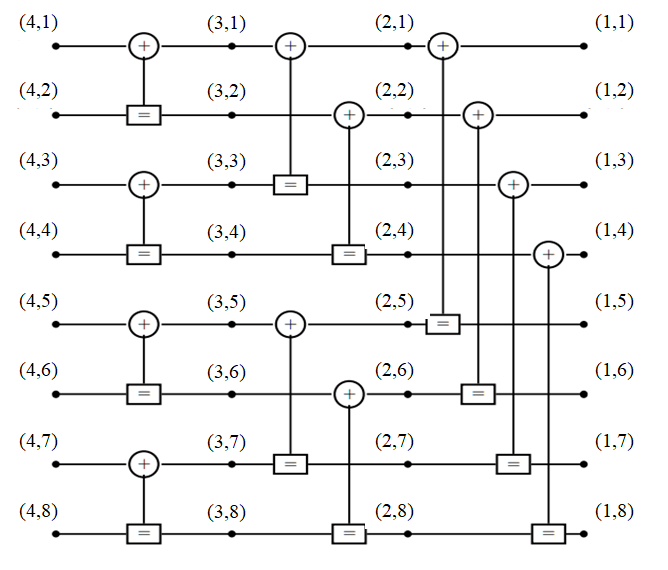
\includegraphics[width=12cm]{fig/graph_presentation.png}
 \caption{The graph factor for polor code, $N=8, n=3$.}
 \label{fig:graph_presentaion}
\end{figure}

\begin{figure}
 \centering
 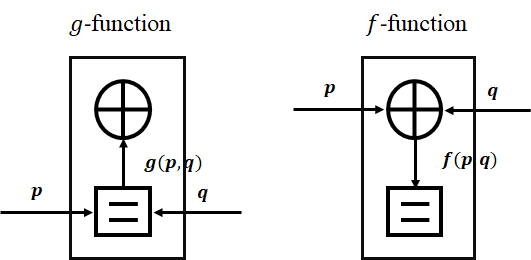
\includegraphics[width=10cm]{fig/BCB_function.png}
 \caption{The message passing function in factor graph.}
 \label{fig:BCB function}
\end{figure}



\paragraph{$f$-function}

When the two input messages vectors ${\bf p} = [ \ p_0 \ p_1 \ p_2 \ p_3 \ ]$ and ${\bf q} = [ \ q_0 \ q_1 \ q_2 \ q_3 \ ]$ arrive at the BCB upper branches $s(n)$, the probability that $s(n)=S[l]$ with $l \in \{0 ,1, 2, 3\}$ is given by
\begin{align}
 \text{Pr}\{s(n)=S[l]|{\bf p}, {\bf q}\} & = \frac{\text{Pr}\{{\bf p}, {\bf q}|s(n)=S[l]\}\text{Pr}\{s(n)=S[l]\}}{\text{Pr}\{{\bf p}, {\bf q}\}} \nonumber \\
 & = \frac{\text{Pr}\{s(n)=S[l]|{\bf p}\}\text{Pr}\{s(n)=S[l]|{\bf q}\}\text{Pr}\{{\bf p}\}\text{Pr}\{{\bf q}\}}{\text{Pr}\{{\bf p}, {\bf q}\}} \nonumber \\
 & = \beta p_l q_l ,
\end{align}
where
\begin{align}
 \beta = \frac{\text{Pr}\{{\bf p}\}\text{Pr}\{{\bf q}\}}{\text{Pr}\{{\bf p}, {\bf q}\}} = \frac{1}{p_0 q_0 + p_1 q_1 + p_2 q_2 + p_3 q_3} ,
\end{align}
is a normalization factor. Therefore, the output message is
\begin{align}
 f({\bf p}, {\bf q}) = \beta [ \ p_0 q_0 \ p_1 q_1 \ p_2 q_2 \ p_3 q_3 \ ] .
\end{align}

\paragraph{$g$-function}
	
A specific parity-check equation is satisfied if the $\mathbb{F}_4$ sum of the connected quaternary symbols in the corresponding Tanner graph is equal to zero, i.e., $s(n) \oplus s(n_1) \oplus s(n_2) = 0$. Assuming that the two input messages derived from the variable nodes $s(n_1)$ and $s(n_2)$ are ${\bf p} = [ \ p_0 \ p_1 \ p_2 \ p_3 \ ]$ and ${\bf q} = [ \ q_0 \ q_1 \ q_2 \ q_3 \ ]$, respectively. The probability that the parity-check equation is satisfied under the the assumption that $s(n)=S[0]$ is
\begin{align}
 \text{Pr}\{s(n)=S[0]|{\bf p}, {\bf q}\} = & \quad \text{Pr}\{s(n_1)=S[0], s(n_2)=S[0]|{\bf p}, {\bf q}\} \nonumber \\
 & + \text{Pr}\{s(n_1)=S[1], s(n_2)=S[1]|{\bf p}, {\bf q}\} \nonumber \\
 & + \text{Pr}\{s(n_1)=S[2], s(n_2)=S[2]|{\bf p}, {\bf q}\} \nonumber \\
 & + \text{Pr}\{s(n_1)=S[3], s(n_2)=S[3]|{\bf p}, {\bf q}\} \nonumber \\
 = & \quad p_0 q_0 + p_1 q_1 + p_2 q_2 + p_3 q_3.
\end{align}
Similarly we can have
\begin{align}
 \text{Pr}\{s(n)=S[1]|{\bf p}, {\bf q}\} & = p_0 q_1 + p_1 q_0 + p_2 q_3 + p_3 q_2, \nonumber \\
 \text{Pr}\{s(n)=S[2]|{\bf p}, {\bf q}\} & = p_0 q_2 + p_2 q_0 + p_1 q_3 + p_3 q_1, \nonumber \\
 \text{Pr}\{s(n)=S[3]|{\bf p}, {\bf q}\} & = p_0 q_3 + p_3 q_0 + p_1 q_2 + p_2 q_1.
\end{align}
Finally, the message out of one check node equals
\begin{equation}
 \text{CHK}({\bf p},{\bf q})= \left[
 \begin{split}
  &p_0 q_0 + p_1 q_1 + p_2 q_2 + p_3 q_3 \\
  &p_0 q_1 + p_1 q_0 + p_2 q_3 + p_3 q_2 \\
  &p_0 q_2 + p_2 q_0 + p_1 q_3 + p_3 q_1 \\
  &p_0 q_3 + p_3 q_0 + p_1 q_2 + p_2 q_1
 \end{split}
 \right]^T.
\end{equation}


\subsubsection{General Sum Product Algorithm decoder}


	In addition to SCL decoder, SPA decoder can also be used to decode polar code. We can replace this SPA decoder with the G-SPA decoder, e.g., passing APP vector in factor graph by $f$ and $g$ functions. It can be easily converted separated channel decoding into joint channel decoding GDMA (JCD-GDMA) system.  
	
\paragraph{Initialization}
	
	In G-SPA, we changed the LLR representation to vector representation, and before message passing, we need to set the initial vectors. For simplicity, we set the initial vectors on the most left as the initial APPs of the received superimposed signal. The rightest vectors are determined according to the frozen bits of the polar code, and the other vectors are the message.

The rightmost nodes $(1, j)$ are associated with channel input vectors that are observed through a noisy channel, $1 \leq i \leq n+1, 1 \leq j \leq N$ where $N$ is the codeword length. 
\begin{align}
L_{1,j} = [p_0 \quad p_1 \cdots p_L]. \quad p_l = \text{Pr}\{s=S[l]|r\}
\end{align}

The leftmost nodes, $(n+1, j)$, are associated with the source data that are to be estimated. If $u_j$ is a frozen bit, we can determine that the leftmost $R_{n+1.j}$ is equal to the superimposed signal $S[0]$, so it can be represented as


\begin{equation}
R_{n+1.j}
\nonumber \\ = 
\left\{
             \begin{array}{lr}
             { [1 \quad 0 \quad \cdots \quad 0] }, \ \text{if  is a frozen coordinate} &  \\
           { [ \frac{1}{L} \quad \frac{1}{L} \quad \cdots \quad \frac{1}{L} ] },  \ \text{if  is an infrozen coordinate}& \\ 
             \end{array}
\right.
\end{equation}

All the other nodes $R_{i.j}$ and $L_{i.j}$ are setted equal to $[\frac{1}{L} \quad \frac{1}{L} \quad \cdots \quad \frac{1}{L}]$ 


\begin{figure}[t!]
 \centering
 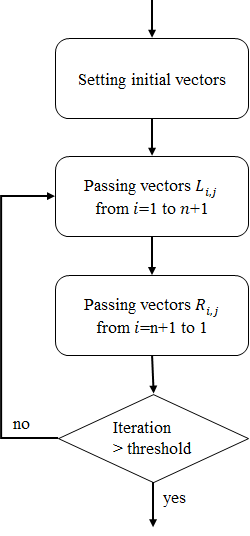
\includegraphics[width=5cm]{fig/polar_gspa_flowchart.png}
 \caption{The flow chart of polar code G-SPA decoder.}
 \label{fig:polar_gspa_flowchat}
\end{figure}

\paragraph{Message passing}

	After setting initial vectors of the factor graph, the massage passing procedure is as fig.\ref{fig:polar_gspa_flowchat}. Unlike the SCL decoder, all operations in the SPA decoder are parallel. The operations will start from the rightmost nodes, then pass the message vectors to the left in sequence. Until updating to the leftmost node, and then act to the right nodes. When it updates to the rightmost nodes again, it finishes an iteration. The BCB calculation is described as

\begin{align}
L_{i+1,\ j} = f \{ L_{i, \ j + N_i}, \ g\{L_{i, \ j}, R_{i, \ j} \} \} \nonumber \\
L_{i+1, \ j+N_i} = g \{ L_{i, \ j + N_i}, \ f\{L_{i, \ j}, \  R_{i+1, \ j} \} \} \nonumber \\
R_{i, \ j} = f \{ R_{i+1, \ j}, \ g\{L_{i, \ j+N_i}, \ R_{i+1, \ j+N_i} \} \} \nonumber \\
R_{i, \ j+N_i} = f \{ R_{i+1, \ j+N_i}, \ g\{L_{i,j}, \ R_{i+1, \ j} \} \} 
\end{align}
, where $N_i=2^{n-i}$ is the connection between each nodes.


\paragraph{Simulation result}

 We now compare the decoders using SPA and using G-SPA. The BLER performances of GDMA-JCD and GDMA-SCD systems using a (256, 128) rate-1/2 Polar code with BPSK transmissions over quasi-static Rayleigh flat-fading channels are provided in Fig.~\ref{fig:bler_polar_spa}. The maximum number of decoding iterations is set to 50 for both SPA and G-SPA. In the transmissions over block flat-fading channels, the GDMA-JCD scheme outperforms the GDMA-SCD scheme in low-SNR region, and the performances of two schemes converge to each other in high-SNR region. Since the block fading systems are lack of channel diversity, e.g., the probability of deep fading is very high, and the coding gain is not obvious. Hence, we further consider an OFDM-GDMA system that can obtain channel diversity from each sub-carrier using a (1024, 512) rate-1/2 Polar code that has $16$ sub-carrier and $64$ bits for each sub-carrier symbol. The BLER performance of GDMA-OFDM-JCD and GDMA-OFDM-SCD using the same parameters as above and are provided in Fig.\ref{fig:bler_ofdm_polar_spa}. We found that JCD can effectively use different user information, even when increasing the number of users, performance has almost no loss.

\begin{figure}[H]
 \centering
 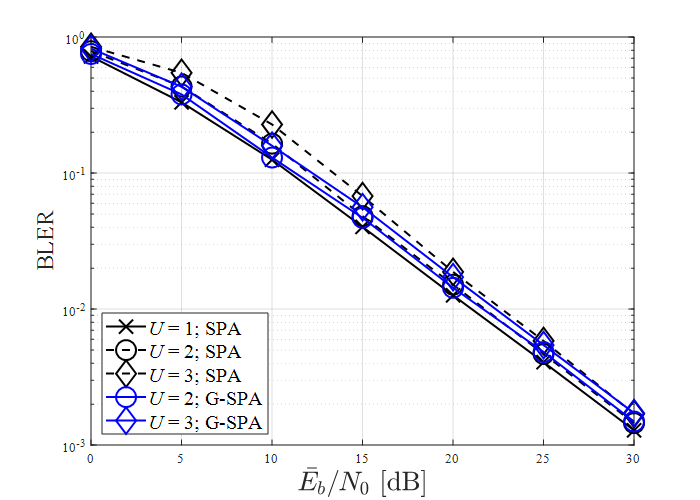
\includegraphics[width=14cm]{fig/bler_polar_spa.png}
 \caption{BLER performances of (256, 128) Polar-coded GDMA systems over quasi-static Rayleigh flat-fading channels.}
 \label{fig:bler_polar_spa}
\end{figure}

\begin{figure}[H]
 \centering
 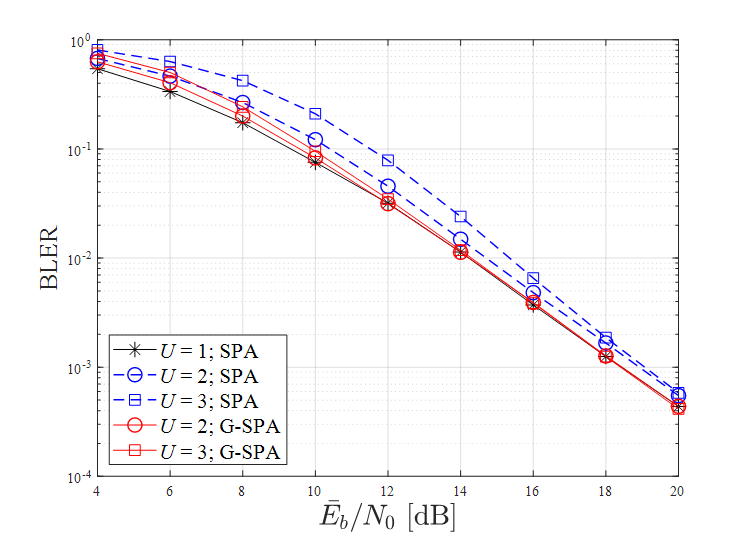
\includegraphics[width=14cm]{fig/bler_gdma_ofdm_polar_spa.png}
 \caption{BLER performances of (1024, 512) Polar-coded GDMA OFDM systems over quasi-static Rayleigh flat-fading channels with 16-subcarrier.}
 \label{fig:bler_ofdm_polar_spa}
\end{figure}

\subsubsection{Joint Successive Cancellation List decoder}

 There are some well-known decoders such as SPA\cite{arikan2010polar}, SCL \cite{scl15}, and SCAN for polar codes. These decoders have their advantages, such as SPA decoder, which is very simple in hardware implementation, and SCL with CRC is able to achieve the best performance in AWGN channel. Compared with the parallel operation of the SPA decoder, the SCL decoder's operation is in a specific order. For implementing a joint successive cancellation list (J-SCL)decoder, we still use $\bf{L_{i,j}}$  $\bf{R_{i,j}}$  to represent the message vectors and $f$-function $g$-function as the operation calculator where $g$-function a vector product calculation, $f$-function a vector parity check calculation. 

Before message passing, we need to set the initial vectors. For simplicity, we set the initial vectors on the rightmost nodes as the  APPs of the superimposed signals. Compared to the G-SPA decoder, the J-SCL decoder does not initialize the other node values.

The rightmost nodes (n+1, j) are associated with channel input vectors $\bf{p}$ that are observed through a noisy channel. 
\begin{align}
{\bf{L_{i,j}}} = [p_0 \quad p_1 \cdots p_L]. \quad {\bf{p_l}} = \text{Pr}\{s=S[l]|r\}
\end{align}

\paragraph{Update for odd branch}

Fig.\ref{fig:jscl_uplayer} and equ. \ref{equ:scl_odd} show a basic computation unit for odd channels. The vectors passing to odd channels can be computed via recursion until leftmost nodes. If passing to the leftmost unfrozen nodes, it will map to the LLR value $e_{\text{LLR}}[c_{j,u}]$ according to mapping rules in chapter-\ref{c:gdma} and obtain a message bit $\hat{u}_{j,u}$ that is the hard decoding value for the $j$-th codeword and $u$-user.

\begin{align}
{\bf{L_{i+1,j}}} = f({\bf L_{i,j}, \ L_{i,j+N_t}})
\label{equ:scl_odd}
\end{align}

\begin{figure}[H]
 \centering
 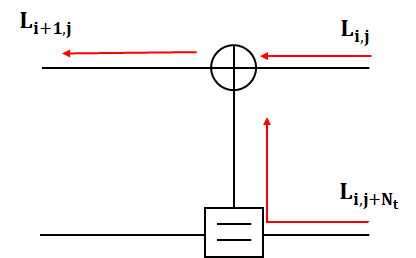
\includegraphics[width=8cm]{fig/jscl_uplayer.png}
 \caption{The factor graph of J-SCL upper layer (even branch) message passing.}
 \label{fig:jscl_uplayer}
\end{figure}


\paragraph{Update for even branch}
Fig.\ref{fig:jscl_lowlayer} and equ.\ref{equ:scl_even} show a basic computation unit for even channels. The vectors passing for even channels can also be computed via recursion. Instead of passing soft right propagating vectors $R_{i+1,j}$ in the G-SPA decoder, the vectors $\bf R_{i+1,j}$ are hard feedback vectors according to message bits $\hat{u}_{j,u}, u \in \{ 1, \cdots, U\}$.

\begin{align}
{\bf{L_{i+1,j+N_i}}} = g( {\bf{L_{i+1,j+N_i}}}, \ f ({\bf{ L_{i+1,j}}} , {\bf{R_{i+1,j}}}) )
\label{equ:scl_even}
\end{align}

Assume that $U=2$ and BPSK transmission, the feedback vectors $\bf R_{i+1,j}$ are described as : 
\begin{align}
\text{if} \  \hat{u}_{j,1}= 0 \ \text{and} \ \hat{u}_{j,2}= 0, {\bf R_{n+1,j}} = {[1 \ 0 \ 0 \ 0]} \nonumber \\
\text{if} \  \hat{u}_{j,1}= 0 \ \text{and} \ \hat{u}_{j,2}= 1, {\bf R_{n+1,j}} = {[0 \ 1 \ 0 \ 0]} \nonumber \\
\text{if} \  \hat{u}_{j,1}= 1 \ \text{and} \ \hat{u}_{j,2}= 0, {\bf R_{n+1,j}} = {[0 \ 0 \ 1 \ 0]} \nonumber \\
\text{if} \  \hat{u}_{j,1}= 1 \ \text{and} \ \hat{u}_{j,2}= 1, {\bf R_{n+1,j}} = {[0 \ 0 \ 0 \ 1]} \nonumber 
\end{align}



\begin{figure}[H]
 \centering
 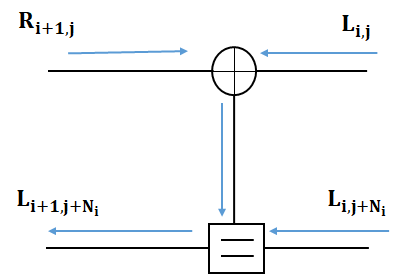
\includegraphics[width=8cm]{fig/jscl_lowlayer.png}
 \caption{The factor graph of J-SCL lower layer (odd branch) message passing.}
 \label{fig:jscl_lowlayer}
\end{figure}

Once obtain $\bf{R_{n+1,j}}$ from the leftmost nodes, we can also derive right propagating vectors $\bf{R_{i,j}}$ via recursion as

\begin{align}
{\bf{R_{i,j}}} = f ( \bf R_{i+1,j} , R_{i+1,j+N_i}) ) \nonumber  \\
\bf{R_{i,j+N_i}} = R_{i+1,j+N_i}  \nonumber
\end{align}
 

\paragraph{Metric path}

After obtain the leftmost probability vectors, we convert probability vectors to the LLR values $e_{\text{LLR}} [c_{j,u} ]$  where $u \in \{1,2,…,U\}  j \in \{1,2,…,N\}$ of each user, which can be obtained by the above formula. Besides, we must record the PM value of this period where PM value is used in list decoding to record the LLR value of each metric path. SCL decoder will only have two forks per path, which are LLR values equal to 0 or 1  respectively. Different from SCL decoder, the forks of each J-SCL path is $L = 2^{mU}$ since the path metric $\text{PM}_l^i$ must contain each user hard decoding information, where $L$ is the number of superimposed signals, we can express the expression as follows:

For the $l$-th path and the $i$-th level, $i=1,2,\cdots,N$, the PM value is given by


\begin{align}
\text{PM}_l^i \triangleq \sum_{j=1}^{i} \sum_{u=1}^{U} \text{ln} \{ 1+\text{exp}[-(1-2 \hat{u}_{j,u} ) e_{\text{LLR}})] \}
\end{align}
where $\hat{u}_{j,u}$ are the hard decoding value for the $j$-th codeword and $u$-th user according to $e_\text{LLR} [c_{j,u} ]$. 

\paragraph{Simulation result}
The BLER performances of GDMA-JCD and GDMA-SCD systems using a (256, 128) rate-1/2 Polar code with CRC-16 BPSK transmissions over quasi-static Rayleigh flat-fading channels are provided in Fig.~\ref{fig:bler_polar_scl}. The maximum number of decoding iterations is set to 50 for both SPA and G-SPA. In the transmissions over block flat-fading channels, the GDMA-JCD scheme outperforms the GDMA-SCD scheme in low-SNR region, and the performances of two schemes converge to each other in high-SNR area. We further consider an OFDM-GDMA system using a (1024, 512) rate-1/2 Polar code with CRC-16 that has $16$ sub-carrier and $64$ bits for each sub-carrier symbol. The BLER performance of GDMA-OFDM-JCD and GDMA-OFDM-SCD using the same parameters as above and are provided in Fig.~ \ref{fig:bler_ofdm_polar_scl}. We found that JCD can effectively use different user information, even when increasing the number of users, performance has almost no loss.

\begin{figure}[b!]
 \centering
 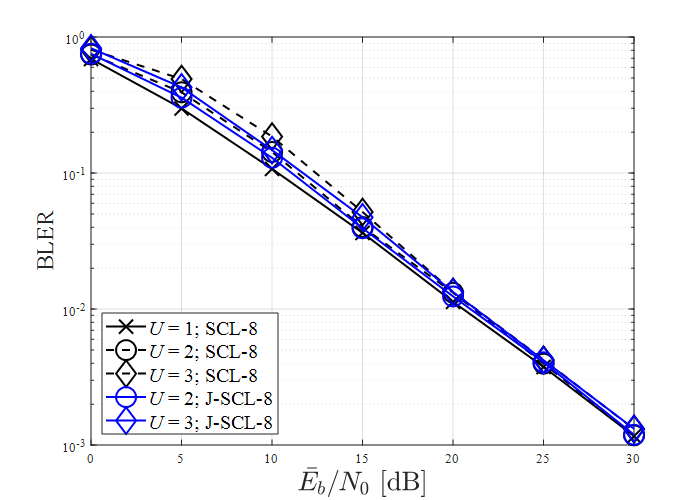
\includegraphics[width=14cm]{fig/bler_polar_scl.png}
 \caption{BLER performances of (256, 128) Polar-coded GDMA systems over quasi-static Rayleigh flat-fading channels.}
 \label{fig:bler_polar_scl}
\end{figure}


\begin{figure}[t!]
 \centering
 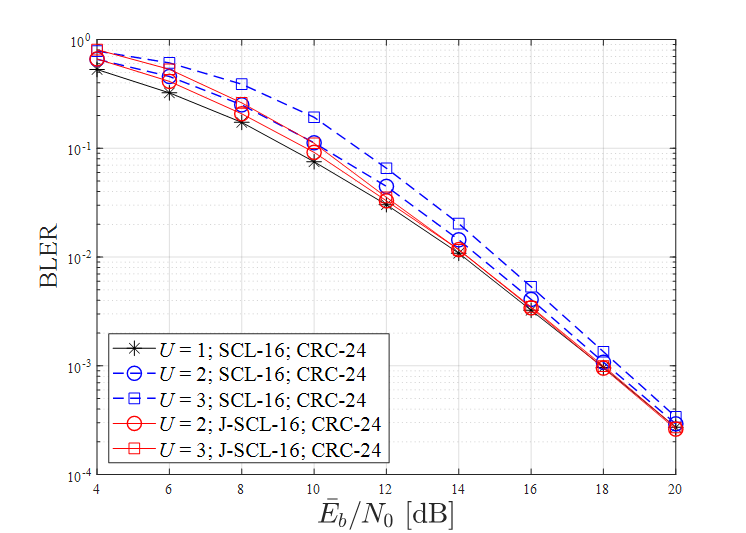
\includegraphics[width=14cm]{fig/bler_gdma_ofdm_polar_scl.png}
 \caption{BLER performances of (1024, 512) Polar-coded GDMA OFDM systems over quasi-static Rayleigh flat-fading channels with 16-subcarrier.}
 \label{fig:bler_ofdm_polar_scl}
\end{figure}

\begin{figure}[b!]
 \centering
 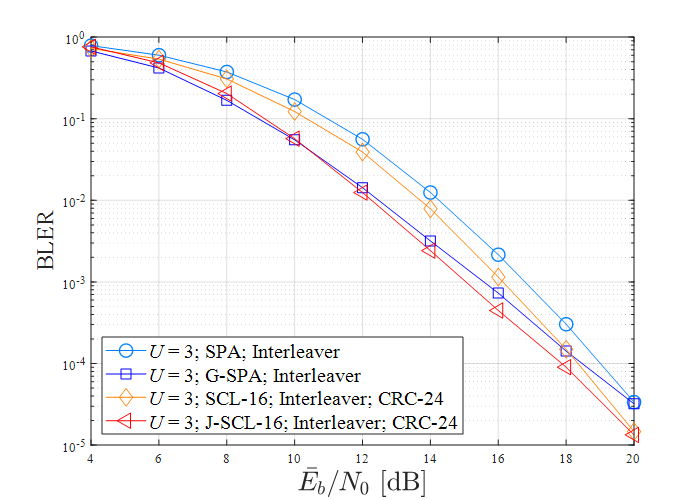
\includegraphics[width=14cm]{fig/bler_gspa_jscl_u3.png}
 \caption{BLER performances of Polar-coded GDMA OFDM systems over quasi-static Rayleigh flat-fading channels with 16-subcarrier and interleaver.}
 \label{fig:bler_ofdm_polar_scl_gspa}
\end{figure}


Since the polar construction is based on the same SNR of received signals, the received signals from OFDM system are distinct according to different energy of each sub-carrier channel gains. Hence, it can use interleaver to force the received signals into similar SNR, and the details were discussed in the paper \cite{lee2019curve}. In fig.\ref{fig:bler_ofdm_polar_scl_gspa}, we compare the performance of G-SPA and J-SCL decoder for polar code and assume code length of 1024, 16 sub-carrier OFDM system, $U=3$. Besides, add the interleaver to make the received massage to avoid sub-block deep fading. Then, add CRC check to SCL and J-SCL for better performance, where CRC length 24 is same as paper \cite{niu2012crc}. We can find that the JCD decoder's performance is better than SCD decoders from 4 dB to 18 dB, and different type decoders will converge in different performance in high SNR. 


